\documentclass[conference]{IEEEtran}

\usepackage[T1]{fontenc}
\usepackage[utf8]{inputenc}
\usepackage{amsmath,amssymb}
\usepackage{graphicx}
\usepackage{subcaption}
\usepackage{booktabs}
\usepackage{siunitx}
\usepackage{url}
\usepackage[hidelinks]{hyperref}
% Sin esto, url usa Courier en T1 (pcrr8t) y pdflatex lo genera como bitmap:
% es el 'mktextfm pcrr8t' que aparece en missfont.log.
\urlstyle{same}

\sisetup{separate-uncertainty=true,detect-all=true}
\DeclareSIUnit\electron{e^-}
\DeclareSIUnit\pixel{px}
\DeclareSIUnit\adu{ADU}
\graphicspath{{img/}}

\begin{document}

\title{Characterization of an 8-bit Monochrome CCD:\\}

\author{\IEEEauthorblockN{Nicol\'as Seguel}
\IEEEauthorblockA{Laboratorio de Instrumentación Astronómica -- IEE3873\\
Pontificia Universidad Cat\'olica de Chile\\
\texttt{neseguel@uc.cl}}}

\maketitle

\section{Introduction}

The detector characterized in this experiment is a DMK 21AU04.AS camera, a monochrome CCD built around a Sony ICX098BL sensor of $640 \times 480$ pixels of \SI{5.6}{\micro\meter}, digitized to 8 bits in Y800 format. The purpose of the session was to measure the parameters that describe the detector as a photon-counting device: bias level, read-out noise (RON), conversion factor, dark current, linearity, photo-response non-uniformity (PRNU), the number of defective pixels, and the presence of persistence\cite{guide}.

The 8-bit depth is the constraint that shapes measurements: the quantization noise, $1/\sqrt{12} = \SI{0.289}{\adu}$, is not negligible against the quantities being measured. A first attempt with the factory settings produced bias frames that were identically zero. The working point was therefore set experimentally (gain 700, brightness 60, gamma 1.00) so that the bias spans several codes, and held fixed for every set, since the conversion factor and the master bias are valid at one setting only.

\section{Theoretical Framework}
\label{sec:theory}

A monochrome frame is a matrix of $n$-bit numbers built from three additive contributions\cite{guide},
\begin{equation}
ADU_{i,j} = \alpha \left( BIAS_{i,j} + DARK_{i,j}\,\Delta t
+ \eta_{i,j} I_{i,j}\,\Delta t \right),
\label{eq:model}
\end{equation}
where $\alpha$ is the conversion factor in ADU per electron, $\Delta t$ the integration time and $\eta$ the quantum efficiency. Each calibration frame isolates one term: a bias is taken with $I = 0$ and $\Delta t \to 0$, a dark with $I = 0$, and a flat with $I$ constant. Results are quoted with the inverse factor $K = 1/\alpha$ [e$^-$/ADU], which converts a signal into electrons directly.

Propagating the variances of \eqref{eq:model}, with the dark and photon terms
Poissonian, gives $\sigma^2(ADU) = \alpha^2 [\,\sigma^2_{BIAS} + DARK\,\Delta t + \eta I \Delta t\,]$. The RON is therefore measured on the \emph{difference} of two bias frames, which cancels the fixed pattern and leaves only temporal noise,
\begin{equation}
\mathrm{RON} = \frac{\sigma(B_1 - B_2)}{\sqrt{2}} ,
\label{eq:ron}
\end{equation}
and the fixed-pattern noise follows from the spatial dispersion of the master bias, $\sigma^2_{M} = \mathrm{FPN}^2 + \mathrm{RON}^2/N$.

In the photon-noise-limited regime the same expression is a straight line between the variance and the signal $S$ of a flat, the photon transfer curve (PTC)\cite{janesick},
\begin{equation}
\sigma^2 = \frac{S}{K} + \mathrm{RON}^2 ,
\label{eq:ptc}
\end{equation}
whose slope gives $K$ and whose intercept gives the RON a second, independent time. Each point comes from a pair of flats at the same $\Delta t$, with $S = \tfrac{1}{2}(\bar{F_1}+\bar{F_2})$ and $\sigma^2 = \mathrm{var}(F_1-F_2)/2$; the difference removes the PRNU. The full well accessible to the digitizer is $255\,K$.

The dark current is the slope $D$ of the dark signal against integration time, $S_{dark} = D\,\Delta t + c$, where $c$ must be compatible with zero if the master bias is correct. Linearity is assessed on the residuals of a straight line fitted to the flat signal versus $\Delta t$, since the direct plot always looks straight, and the PRNU is the spatial dispersion of a normalized flat once the low-frequency illumination pattern has been divided out.

\section{Equipment and Method}
\label{sec:equip}

Table\ref{tab:equip} lists the equipment. The light source for the flat fields was the LED flashlight of a phone, pointed at a white wall and observed out of focus so that the illumination reaching the sensor was smooth; all other measurements were taken in a dark room with the lens cap on.

\begin{table}[htbp]
\caption{Equipment used in the session.}
\label{tab:equip}
\centering
\small
\begin{tabular}{@{}ll@{}}
\toprule
\textbf{Item} & \textbf{Use} \\
\midrule
DMK 21AU04.AS (Sony ICX098BL) & detector under test \\
Laptop computer & acquisition and analysis \\
AstroDMx Capture 2.18.2 & FITS acquisition \\
Phone LED flashlight & flat-field illumination \\
Dark room & bias, dark and persistence sets \\
\bottomrule
\end{tabular}
\end{table}

Five sets were acquired, all at \SI{24}{\celsius} room temperature and at a fixed working point of gain 700, brightness 60 and unity gamma: 100 bias frames at $\Delta t = \SI{1}{\micro\second}$; 95 darks at seven times between \SI{2}{\second} and \SI{90}{\second}; 120 flats at twelve levels between \SI{5}{\milli\second} and \SI{100}{\milli\second}, from 12ADU to saturation; 120 darks matching every flat integration time, which the PTC requires because subtracting the bias alone leaves the dark term of \eqref{eq:model} inside the signal; and 20 frames taken immediately after saturating the detector. Signal levels are measured on a central region of $200 \times 200$ pixels, because the array is not spatially homogeneous. The read-out noise carries no such restriction, since the difference of two frames removes any fixed structure, and is quoted for the full array.

\section{Results}
\label{sec:res}

\subsection{Bias, read-out noise and defective pixels}

The master bias of the 100 frames sits at \SI{3.09}{\adu} and its histogram, Fig.\ref{fig:bias}, occupies eight codes with a Gaussian dispersion of \SI{1.13}{\adu}. Applying \eqref{eq:ron} to the 50 pairs gives $\mathrm{RON} = \SI{1.125}{\adu}$ over the full array, and the master dispersion gives $\mathrm{FPN} = \SI{0.26}{\adu}$: the read-out noise dominates the fixed pattern by a factor of four. Estimated the other way round, as the temporal dispersion of each pixel over the 100 frames followed by the median over pixels, it gives \SI{1.122}{\adu}. The two routes differ by \SI{0.3}{\percent}, which shows that the noise is stationary in time and uniform over the array. A fraction of \SI{0.50}{\percent} of the pixels still reads zero, which is the lower tail of the distribution being clipped against the bottom of the converter with the offset control already at its maximum.

\begin{figure}[htbp]
\centering
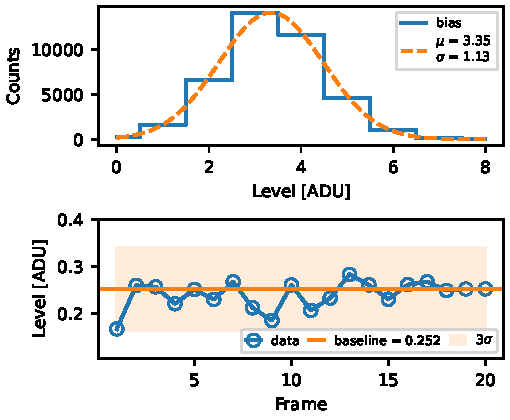
\includegraphics[width=\linewidth]{fig_bias_persistencia.pdf}
\caption{Top: histogram of a bias frame and the Gaussian of equal mean and dispersion; the distribution spans eight codes, the minimum for the RON to be measurable at 8 bits. Bottom: level of the twenty frames taken immediately after saturation, with the baseline and its $3\sigma$ band.}
\label{fig:bias}
\end{figure}

The bad pixel mask, built at $5\sigma$ from the master dark and the normalized master flat, contains 84 pixels (\SI{0.027}{\percent}): 54 hot, 36 noisy and none dead.

\subsection{Conversion factor}

Fig.\ref{fig:ptc} shows the PTC built from the twelve flat levels. Ten points lie on the straight line of \eqref{eq:ptc}; the two highest bend downwards, the signature of pixels clipping against 255ADU, and are excluded. The fit gives
\begin{equation}
K = \num{8.83 \pm 0.04}\si{\electron\per\adu}, \quad R^2 = 0.9998 ,
\end{equation}
an intercept equivalent to $\mathrm{RON} = \SI{1.10}{\adu}$, and a full well of \SI{2252}{\electron} set by the 8-bit converter and not by the physical well. The read-out noise in electrons is \SI{9.94}{\electron} from the bias and \SI{9.72}{\electron} from the PTC intercept.

\begin{figure}[htbp]
\centering
\includegraphics[width=\linewidth]{fig_ptc_dark.pdf}
\caption{Top: photon transfer curve; circles are the points used in the fit, crosses the two saturated levels, the slope is $1/K$ and the intercept $\mathrm{RON}^2$. Bottom: dark signal against integration time. Error bars are the standard error of the frame means, below \SI{0.008}{\adu}, and are therefore contained within the markers.}
\label{fig:ptc}
\end{figure}

\subsection{Dark current}

The dark signal is strictly proportional to the integration time over the whole range measured (Fig.~\ref{fig:ptc}, bottom),
\begin{equation}
D = \num{0.1520 \pm 0.0007}\si{\adu\per\second}
  = \SI{1.343}{\electron\per\pixel\per\second}
\end{equation}
at \SI{24}{\celsius}, and an intercept of \SI{0.27}{\adu}, small compared with the RON. The dark frames are not spatially uniform: Fig.\ref{fig:maps} shows a glow that grows from one corner of the array, reaching \SI{36.6}{\adu} at \SI{90}{\second} against \SI{9.3}{\adu} in the opposite corner. The value quoted above is measured in the central region, away from it.



\subsection{Linearity and PRNU}

The flat signal grows at \SI{2.382}{\adu\per\milli\second} and the residuals stay within \SI{0.74}{\percent} over the range 12--226ADU (Fig.\ref{fig:lin}). The largest residual belongs to the lowest level, where a single ADU of quantization is already \SI{4}{\percent} of the signal; excluding it the bound falls to \SI{0.60}{\percent}. No departure from linearity is detected below saturation, so the operating full well coincides with the digitizer limit.

\begin{figure}[htbp]
\centering
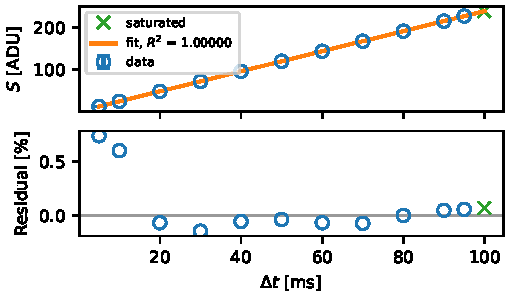
\includegraphics[width=\linewidth]{fig_linealidad.pdf}
\caption{Flat signal against integration time (top) and residuals of the linear fit (bottom). Crosses mark the saturated levels, excluded from the fit.}
\label{fig:lin}
\end{figure}

Separating the normalized flat into a smooth component and a high-frequency one gives a pixel-to-pixel PRNU of \SI{1.07}{\percent}, while the smooth component varies by \SI{21}{\percent} across the field.

\begin{figure}[htbp]
\centering
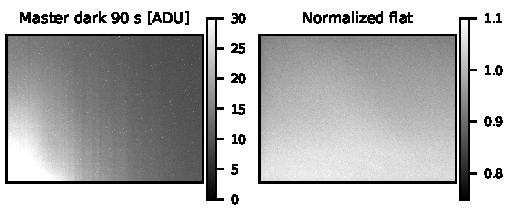
\includegraphics[width=\linewidth]{fig_mapas.pdf}
\caption{Left: master dark of \SI{90}{\second} after bias subtraction, showing the amplifier glow in one corner. Right: master flat normalized to its median; the \SI{21}{\percent} variation is the illumination of the setup.}
\label{fig:maps}
\end{figure}

\subsection{Persistence}

The twenty frames taken after saturating the detector show no remnant signal (Fig.~\ref{fig:bias}, bottom). The first frame lies at \SI{0.166}{\adu}, in fact \emph{below} the baseline of \SI{0.252}{\adu} defined by the last third of the sequence, and the dispersion of the series is \SI{0.030}{\adu}. The result is an upper limit: any persistence is below \SI{0.089}{\adu} at $3\sigma$, that is \SI{0.03}{\percent} of the saturating signal.



Table\ref{tab:summary} collects every result.

\begin{table}[htbp]
\caption{Summary of the measured parameters at \SI{24}{\celsius}, gain 700.}
\label{tab:summary}
\centering
\small
\begin{tabular}{@{}lc@{}}
\toprule
\textbf{Parameter} & \textbf{Value} \\
\midrule
Bias level & \SI{3.09}{\adu} \\
Read-out noise (bias) & \SI{1.125}{\adu} = \SI{9.94}{\electron} \\
Read-out noise (PTC) & \SI{1.10}{\adu} = \SI{9.72}{\electron} \\
Fixed pattern noise & \SI{0.26}{\adu} \\
Conversion factor $K$ & \num{8.83 \pm 0.04}\si{\electron\per\adu} \\
Full well (8-bit ADC) & \SI{2252}{\electron} \\
Dark current & \SI{1.343}{\electron\per\pixel\per\second} \\
Non-linearity & $< \SI{0.74}{\percent}$ (12--226 ADU) \\
PRNU (pixel to pixel) & \SI{1.07}{\percent} \\
Defective pixels & 84 (\SI{0.027}{\percent}) \\
Persistence & $< \SI{0.03}{\percent}$ ($3\sigma$) \\
\bottomrule
\end{tabular}
\end{table}

\section{Discussion}
\label{sec:disc}

The strongest internal check of the measurements is that the read-out noise comes out of two independent routes, the dispersion of the bias differences and the intercept of the PTC, and the two agree to \SI{2.4}{\percent}. The agreement validates the whole reduction chain and confirms that the gain was not disturbed between sets.

Three systematic effects limit the results. The first is the clipping of \SI{0.50}{\percent} of the bias pixels at 0. The offset control was already at its maximum, so the lower tail of the read-out noise distribution could not be recovered. It is also the most likely origin of the \SI{0.27}{\adu} intercept of the dark fit. The second is the amplifier glow, which scales with integration time exactly as the dark signal does and therefore survives the bias subtraction, making the dark current a function of position: the corner rate is about three times the central one. The third is the \SI{21}{\percent} illumination non-uniformity, which belongs
to the setup and not to the sensor, and must be separated from the pixel-to-
pixel term before the PRNU is quoted.

Quantization is the recurring limitation, and it also forces the spatial estimators to be means rather than medians: the median of a master frame always falls on an integer, which turns the dark curve into a staircase and hides the sub-ADU persistence signal entirely.

\section{Conclusions}
\label{sec:concl}

The detector was characterized at \SI{24}{\celsius} with a conversion factor of \num{8.83 \pm 0.04}\si{\electron\per\adu}, a read-out noise of \SI{9.94}{\electron}, a dark current of \SI{1.343}{\electron\per\pixel\per\second} in the central region and a full well of \SI{2252}{\electron} imposed by the 8-bit converter. The response is linear to better than \SI{0.74}{\percent} over the whole usable range, the pixel-to-pixel PRNU is \SI{1.07}{\percent}, \SI{0.027}{\percent} of the pixels are defective, and no persistence is detected above \SI{0.03}{\percent} of the saturating signal.

A repetition would benefit most from two changes: an offset range large enough to keep the bias distribution off the bottom of the converter, and a diffuse extended source in place of the flashlight, which would reduce the \SI{21}{\percent} illumination gradient.

\begin{thebibliography}{1}

\bibitem{guide}
L. Vanzi, \emph{2D Detector Characterization and Image Processing}, course
notes IEE3873, Pontificia Universidad Cat\'olica de Chile.

\bibitem{janesick}
J. R. Janesick, \emph{Photon Transfer: DN $\rightarrow$ $\lambda$}.
Bellingham, WA: SPIE Press, 2007.

\bibitem{astrodmx}
N. Palmer and S. Wainwright, \emph{AstroDMx Capture}, v2.18.2.
\url{https://www.astrodmx-capture.org.uk}

\bibitem{icx}
Sony Corporation, \emph{ICX098BL Diagonal 4.5\,mm (Type 1/4) Progressive Scan
CCD Image Sensor}, datasheet.

\end{thebibliography}

\end{document}
